\appendix
\section{Arduino Code for Line Following Robot}
\subsection{Overview}
The code was programmed using Arduino. Only the .ino, .cpp and config.h files are included in Appendix B. For full code including .h files, access the GitHub: \href{https://github.com/blaketolmie/LFR}{https://github.com/blaketolmie/LFR}
\subsection{LFR\_Main.ino}

\begin{figure}[H]
    \centering
    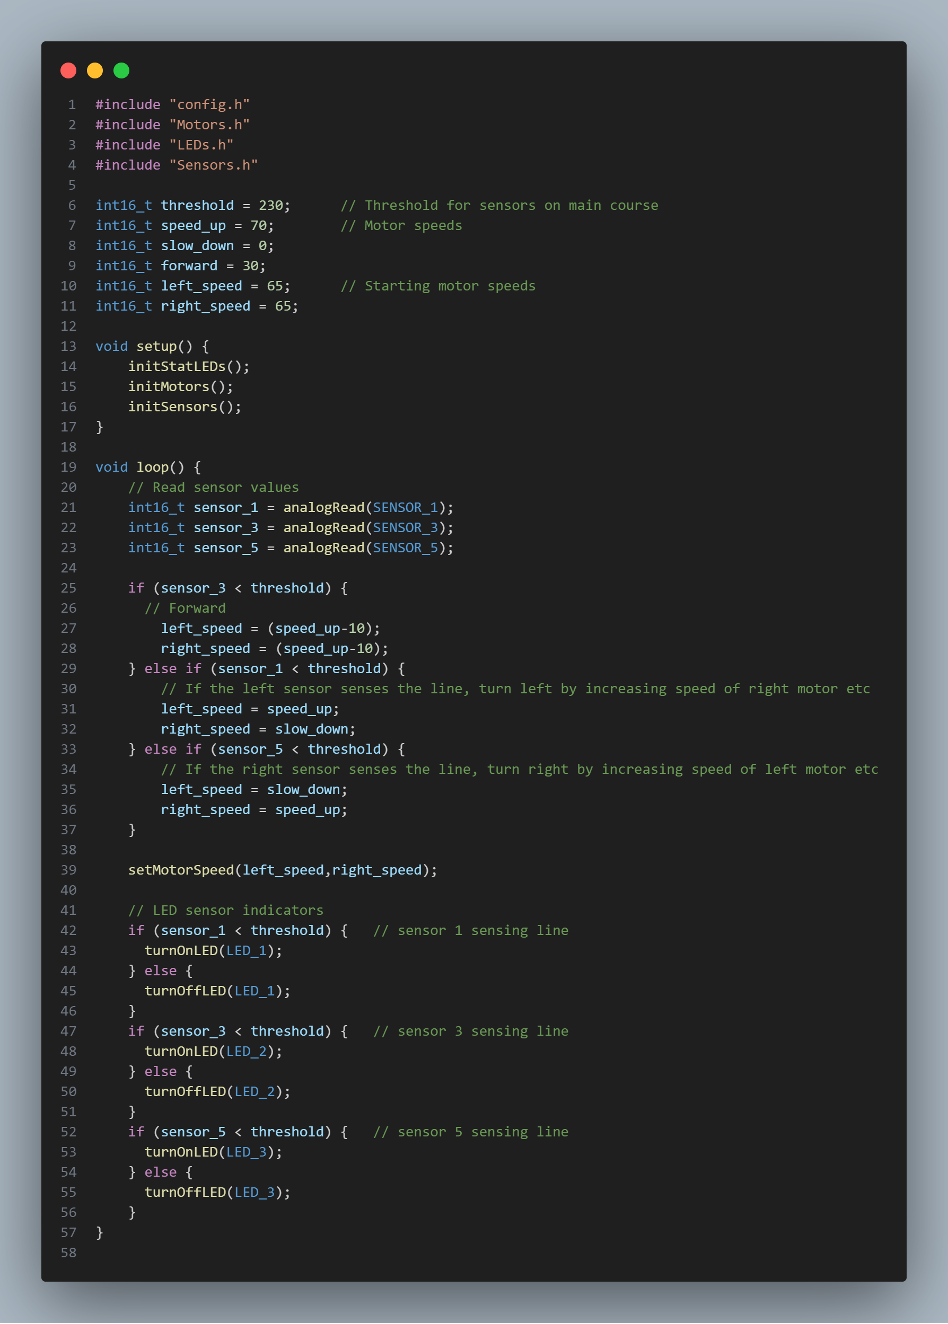
\includegraphics[width=0.8\linewidth]{REPORT/LFR_main.png}
\end{figure}

\subsection{Motors.cpp}

\begin{figure}[H]
    \centering
    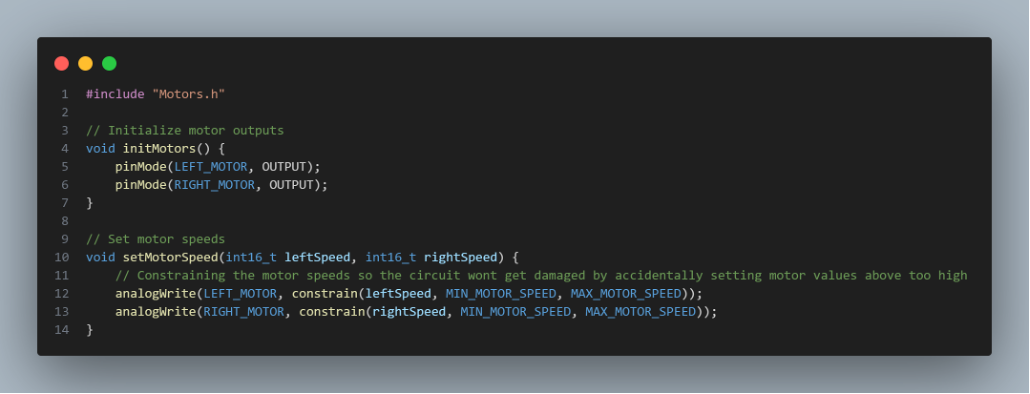
\includegraphics[width=0.8\linewidth]{REPORT/Motorscode.png}
\end{figure}

\subsection{Sensors.cpp}

\begin{figure}[H]
    \centering
    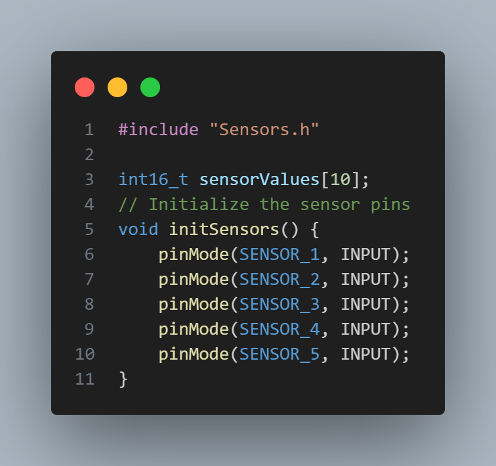
\includegraphics[width=0.8\linewidth]{REPORT/sensorscode.png}
\end{figure}

\subsection{LEDs.cpp}

\begin{figure}[H]
    \centering
    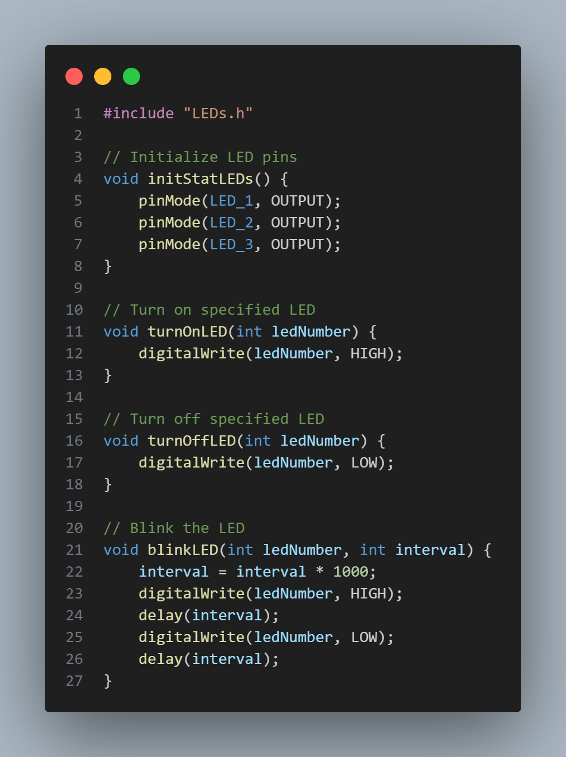
\includegraphics[width=0.8\linewidth]{REPORT/ledscode.png}
\end{figure}

\subsection{Config.h}

\begin{figure}[H]
    \centering
    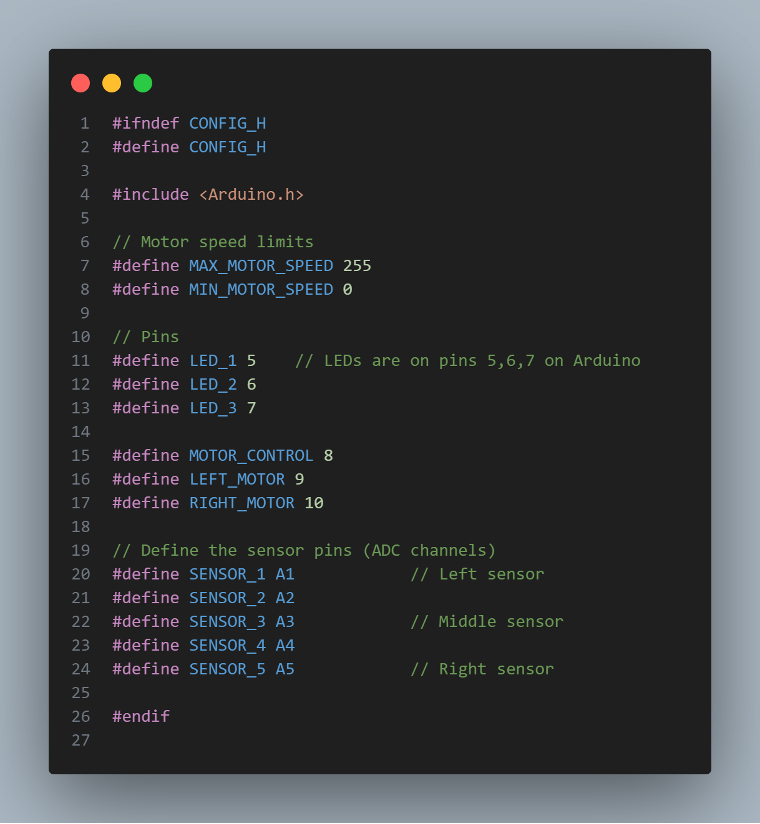
\includegraphics[width=0.8\linewidth]{REPORT/configcode.png}
\end{figure}

\section{Table for LFR Course Times by Sensor Configurations and Weight}
\begin{figure}[H]
    \centering
    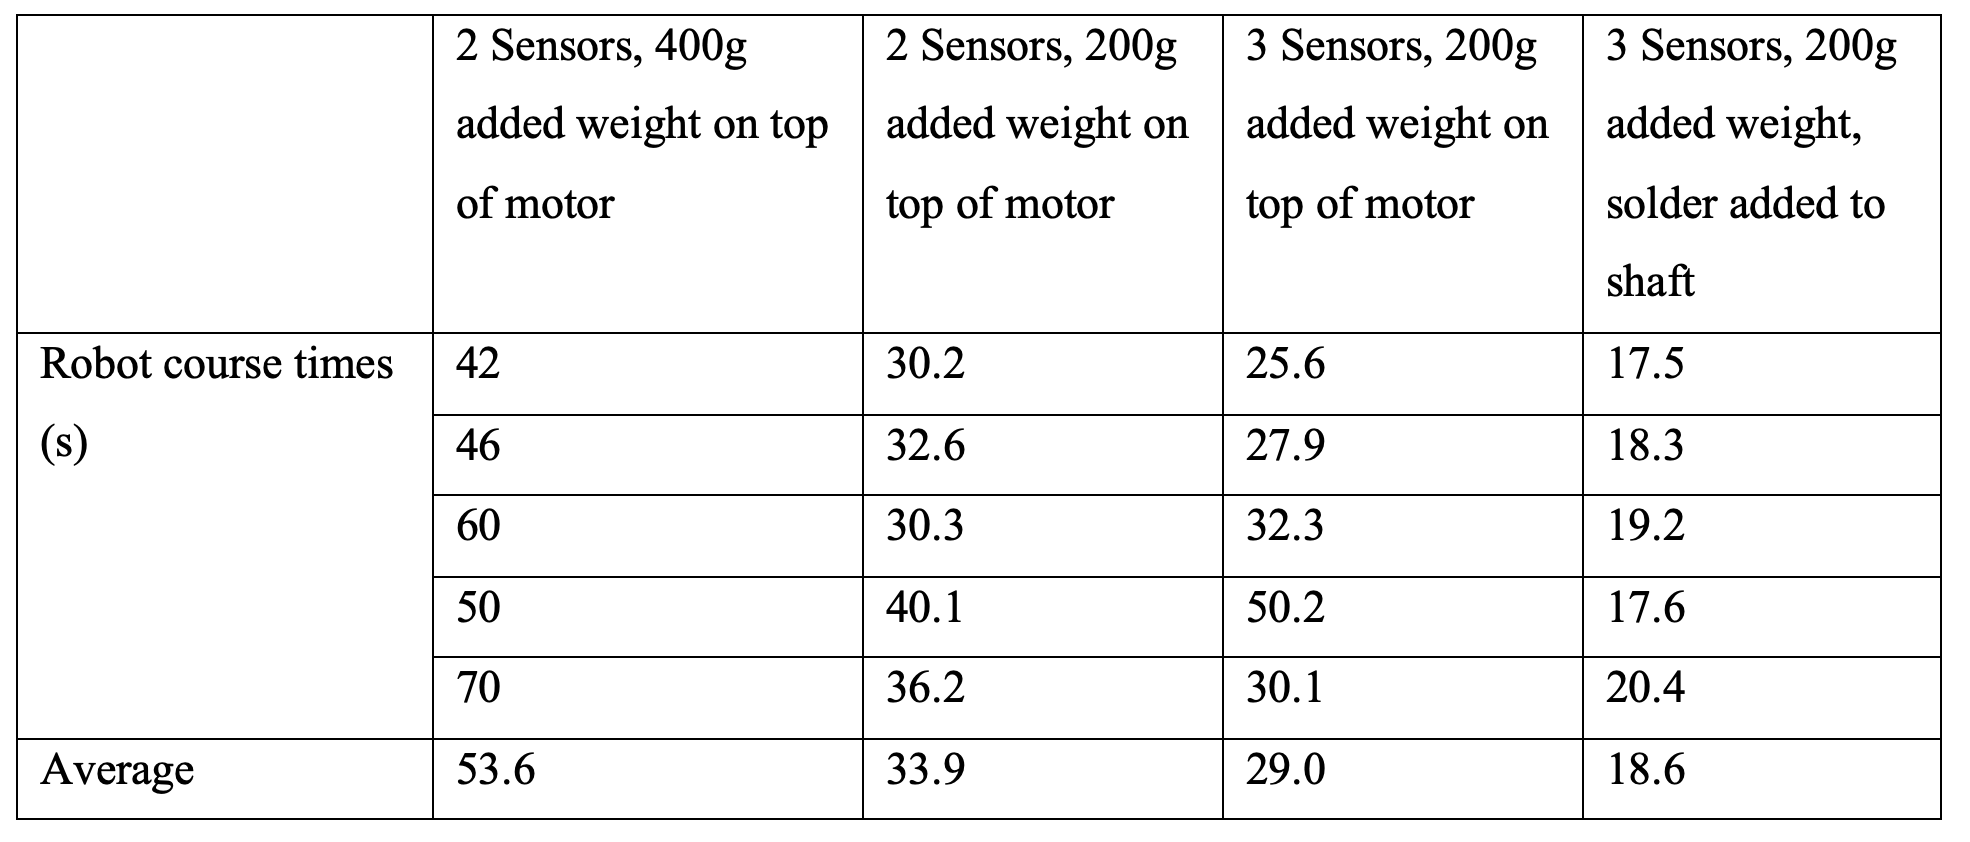
\includegraphics[width=0.8\linewidth]{REPORT/Screenshot 2024-10-20 at 3.11.46 AM.png}
\end{figure}

\section{Allowed Electronic Components}
\begin{figure}[H]
    \centering
    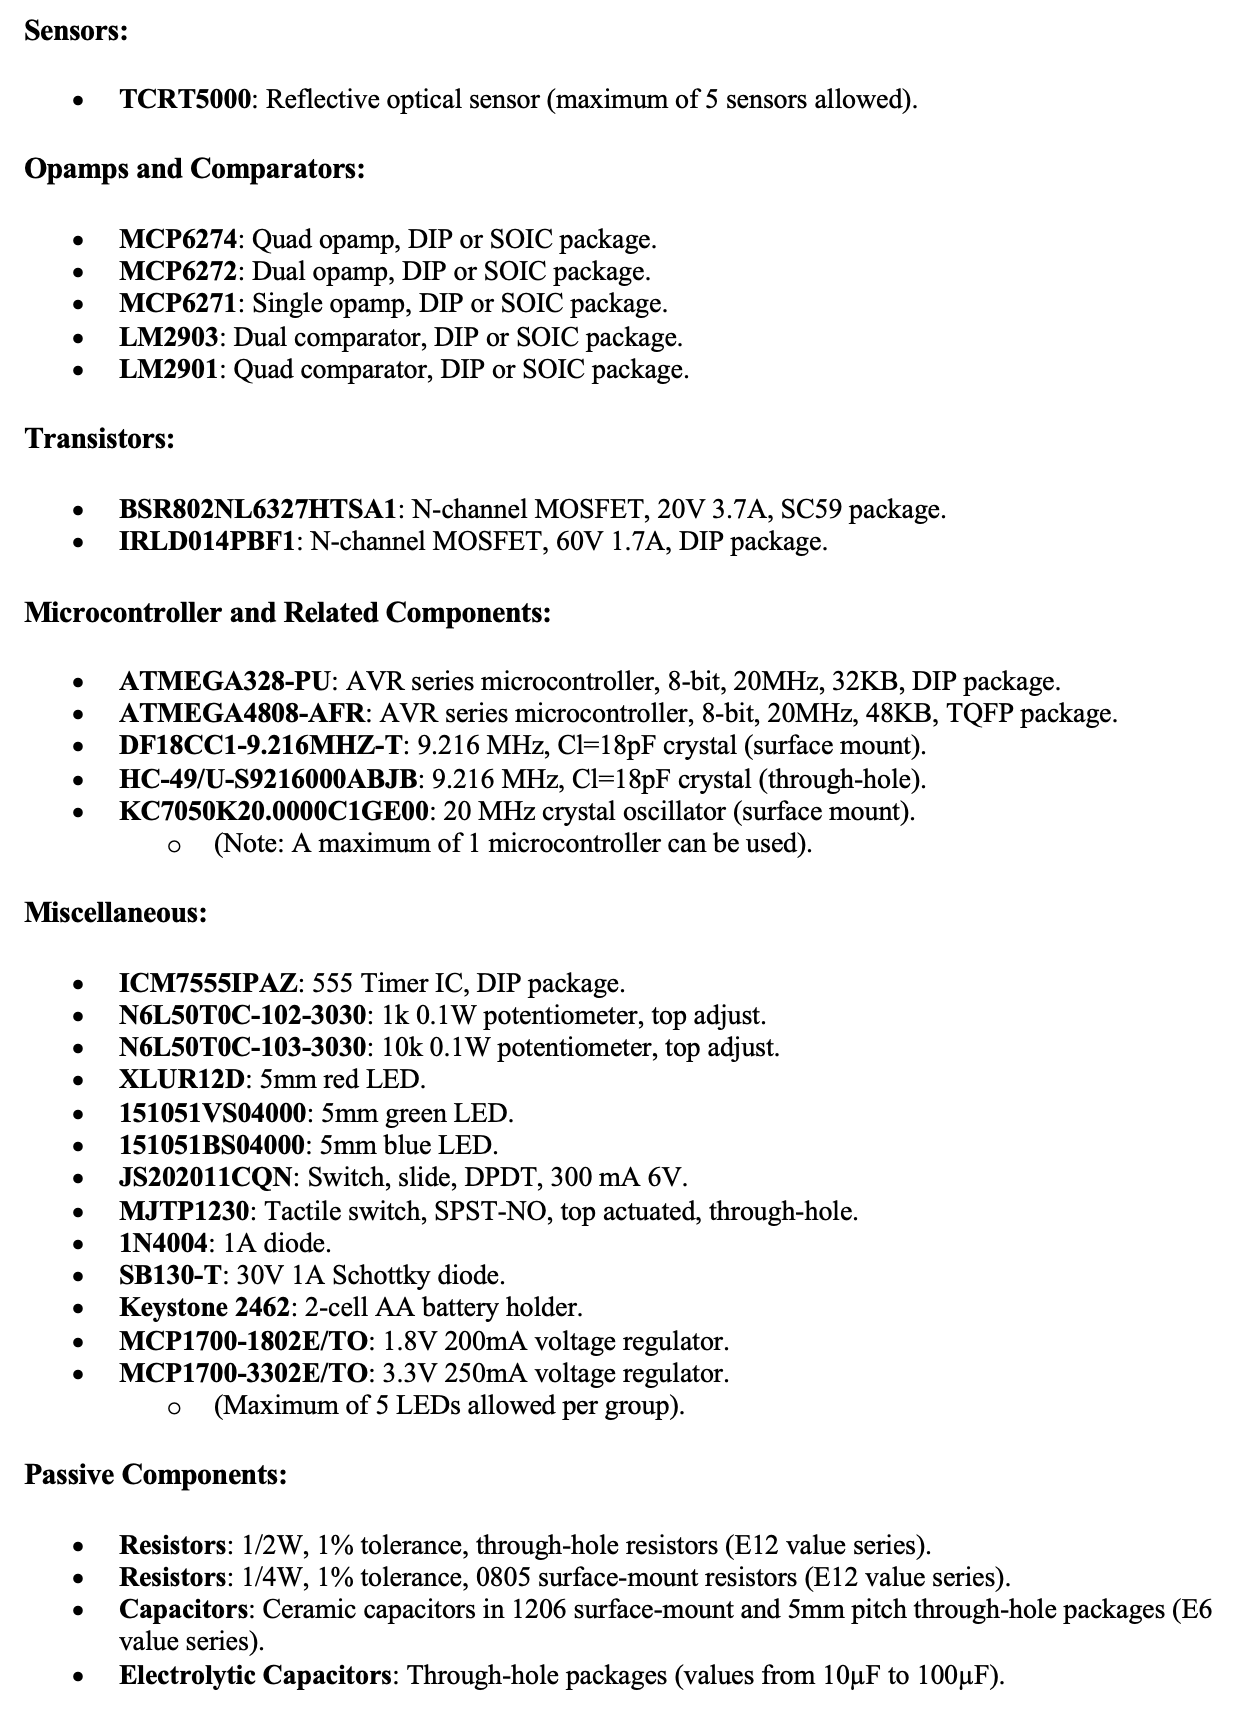
\includegraphics[width=0.8\linewidth]{REPORT/Screenshot 2024-10-20 at 3.10.45 PM.png}
\end{figure}